
%Deprecated duw to restructuring

\chapter{Multi-Agent Stochastic Target Localization}
\workinprogress
This chapter outlines the approach taken to solve the research question stated in the introduction chapter. The context for this problem is derived from the ROCSAFE project \cite{rocsafeNUIG}. \note{Not sure how best to present the problem and how to provide the necessary content to naturally leads to the approaches discussed here. Fill this out further once research questions have been finalized/refined}

%%%%%%%%%%%%%%%%%%%%%%%%%% Bayesian Filtering Sections %%%%%%%%%%%%%%%%%%%%%%%%%%
\section{Bayesian Filtering for State Estimation}
\note{Rename this to stochastic search algorithms or something else}

\subsection{Hidden Markov Models}
\nomenclature[]{HMM}{Hidden Markov Model}
\placeholder{}
\note{Could discuss:
\\Background
\begin{itemize}
    \item What HMMs are
    \item why they're useful in AI
    \item the different commonly used HMMs. 
\end{itemize}
\\ Use in my research:
\begin{itemize}
    \item How the problem can naturally be described by a HMM
    \item Lead into discussion of how DBN is a more natural way to describe the problem and how it leads to efficient factorization of densities for state estimation
\end{itemize}
}
Hidden Markov Models appear frequently in AI literature as they provide an abstract framework to deal with stochastic processes, which themselves are pervasive in their use as a tool to model real-world phenomena. This chapter will outline what HMMs are and their use in literature describing target localization algorithms. A general overview of HMMs can be found in \cite{Murphy1994DynamicLearning}\cite{Ghahramani2001ANNETWORKS}.

\subsubsection{Markov Processes}
It is instructive to understand what is meant by a stochastic process for some of the concepts mentioned in this thesis. The high-level details will be discussed here and the reader can refer to a text on probability theory for a fuller explanation, for example \cite{papoulis02}. A random process can be described as a family of random variables indexed by a set $\tau$: $\{X_t\}_{t\in\tau}$. Commonly in AI, stochastic processes model the evolution of a random system through \textit{discrete} time steps: $\tau$=$\mathbb N$. Common phenomena modelled by stochastic processes include the growth of a bacterial population and the movement of a gas molecule.\par

A first-order discrete-time Markov process is a stochastic process that describes a system which is in a given state at each time step, with the state changing randomly between steps. The steps are elements of the natural numbers and the random process is a mapping from the natural numbers to states. First-order Markov processes have the additional property that the probability distribution of the n$_{th}$ random variable in the process is conditionally independent of all previous probability distributions in the sequence but the $n-1_{st}$: $P(X_t = x_t | X_{t-1} = x_{t-1}, X_{t-2} = x_{t-2}, ... , X_{1} = x_{1}) = P(X_t = x_t | X_{t-1} = x_{t-1})$. This is often referred to as the Markov Property or the memoryless property of Markov processes. In order to describe a Markov process, it is therefore necessary to describe what is known as the transition function between each pair of timesteps: $P(X_t = x_t | X_{t-1} = x_{t-1})$. A common assumption is that the rules that govern state transitions are time invariant, meaning that they can be specified generally for any given pair of timesteps. This assumption will be made for the subsequent discussion. If $X_t$ is a discrete random variable defined over $S$ states, the transition function can be described by a stochastic matrix T, where T$_{i,j}$ = $P(X_t = j | X_{t-1} = i)$: 

\begin{center}
{$\displaystyle \left({\begin{matrix}T_{1,1}&T_{1,2}&\dots &T_{1,j}&\dots &T_{1,S}\\T_{2,1}&T_{2,2}&\dots &T_{2,j}&\dots &T_{2,S}\\\vdots &\vdots &\ddots &\vdots &\ddots &\vdots \\T_{i,1}&T_{i,2}&\dots &T_{i,j}&\dots &T_{i,S}\\\vdots &\vdots &\ddots &\vdots &\ddots &\vdots \\T_{S,1}&T_{S,2}&\dots &T_{S,j}&\dots &T_{S,S}\\\end{matrix}}\right)$}
\end{center}
\par

Some obvious results are worth pointing out; as for any stochastic matrix, by the axioms of probability theory, the sum of conditional probabilities across {$\displaystyle \sum _{j=1}^{S}T_{i,j}=1$} and the transition probabilities over k timesteps can be described by the $k_{th}$ power of the transition matrix: ${(T^k)}_{i,j}$ = $P(X_{t+k} = j | X_{t} = i)$. Markov processes are often described by graphical models, for example Figure \ref{fig:markov-processes}.
\begin{figure}[b]
    \centering
    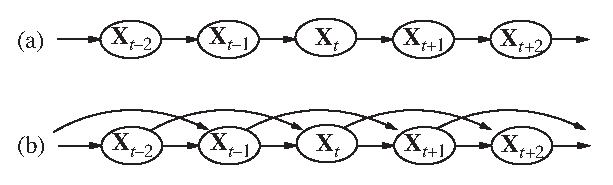
\includegraphics{Chapters/MultiAgentProbabilisticSearch/BayesianFiltering/Figs/markov-processes.eps}
    \caption{First (a) and second (b) order Markov processes \cite{AIAMA}}
    \label{fig:markov-processes}
\end{figure}
It also is possible to calculate the probability of the process experiencing a sequence of states from timesteps 1 as far as t, using the chain rule of probability and the Markov property:
$P(X_{1:t}) = P(X_1, X_2, ..., X_t) = P(X_1)\times P(X_2 | X_1)\times P(X_3 | X_2, X_1) \times P(X_t | X_{t-1}, X_{t-2}, ... , X_1) = P(X_1) \times \prod_{i=2}^{t}{P(X_i | x_{i-1})}$. Marginalization over variables in this sequence allows the calculation of many useful quantities.
\par

\subsubsection{HMM Description}
Hidden Markov Models (HMMs) are models that build on the Markov Process model, which describe the evolution of a random system in the language of probability theory. HMMs assume that the system being modeled can be described by a Markov process, but that the states of this process are unobservable. This means that it isn't possible to determine the state of the system exactly at any given point in time. However, it is possible to make an observation of a random variable that is related to the hidden state which yields information about the hidden state. This is visualised in Figure \ref{fig:hmm}
\begin{figure}[]
    \centering
    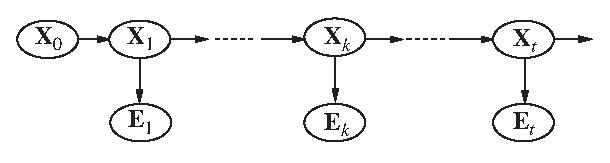
\includegraphics{Chapters/MultiAgentProbabilisticSearch/BayesianFiltering/Figs/smoothing-dbn.eps}
    \caption{A visualisation of a HMM \cite{AIAMA}}
    \label{fig:hmm}
\end{figure}
, where the Markov Process is shown by the variables $X_i$ and the observation variables are shown by variables $E_i$. A HMM can be specified by a triple, $\lambda$ = $(T, O, \pi)$, where $T$ is the stochastic transition matrix, $\pi$ is the initial distribution $P(X_1)$ and O describes the conditional probability of an observation given that the system is in a certain state: $O(E_i, X_i) = P(E_{i} | X_{i})$. Taken together, it is then possible to specify the joint distribution of the hidden state variables and the evidence variables, analogous to the Markov Process: 
$
P(X_{1:t}, E_{1:t}) = P(X_1, X_2, ..., X_t, E_1, E_2, ..., E_t) = P(X_1) \times P(E_1 | X_1) \times
\prod_{i=2}^{t}{(P(X_i | x_{i-1}) \times P(E_t | X_t))}.
$Given representation, it is then possible to answer questions such as:
\begin{itemize}
    \item Given the HMM, $\lambda$, determine the probability of occurrence of a particular observation sequence, $P(E_{1:t} | \lambda)$
    \item Given a sequence of observations $(E_1, E_2, ..., E_n)$, what is the most likely sequence of hidden states that led to these observations? i.e. find \[\argmax_{X_{1:t}} P(X_{1:t} | E_{1:t})\].
    \item Determine the parameters of $T$ and $O$, given a training set of observations, i.e. find the solution to \[\argmax_{\lambda} P(E_{1:t} | \lambda)\].
    \item Filtering: What is the current distribution of the hidden state given all previous evidence ('belief state') of the agent at time t: $P(X_t | E_{1:t})$?
    \item Prediction: What is the distribution of the hidden state in the future, given all evidence to date: $P(X_{t+k} | E_{1:t})$, for some k$>$0?
    \item Smoothing: What is the distribution of a past state given all observations up to the current point in time: $P(X_k | E_{1:t})$, for some 0 $\leq$ k $<$ t?
\end{itemize}
\par

%Might include a subsection on a taxonomy of commonly used HMMs.

\subsubsection{Summary}
In summary, HMMs can be used to abstractly describe the evolution of a stochastic system. They have been used to achieve state of the art performance in problems such as speech recognition \cite{ChiuSTATE-OF-THE-ARTMODELS} and ... . An comprehensive overview of extensions to the vanilla HMM can be found at \cite{Murphy1994DynamicLearning}.
\label{Chapter:HMM}

\subsection{Dynamic Bayesian Networks}
\nomenclature[]{DBN}{Dynamic Bayesian Network}
\nomenclature[]{BN}{Bayesian Network}
\nomenclature[]{CPD}{Conditional Probability Distribution}
\nomenclature[]{2TDBN}{2 Time Slice Dynamic Bayesian Network}

Dynamic Bayesian Networks are a generalization of HMMs and are used to model time series, without being limited to the assumptions of HMMs. The key difference between DBNs and HMMs is that DBNs are not limited in how they decompose the state of a complex stochastic system into the variables that represent its constituent distributions \cite{AIAMA}. Technically, every DBN can be represented as a HMM and visa versa, however, the number of parameters that need to be detemined to represent DBNs can be significantly less that that of HMMs. This is due to the fact that specifying a full joint discrete distribution can require an exponential number of probabilities, whereas specifying the same joint distribution as factored conditional distributions may require far fewer.

\subsubsection{A Note on Bayesian Networks}
A Bayesian Network (BN) is a graphical way to represent a particular factorization of a joint distribution. For a detailed explanation, the reader is referred to \cite{KollerPGM}. To fully explain a complex system, it is often natural to model it as the joint distribution of a number of random variables. This is in general intractable \cite{KollerPGM}. In order to circumvent this, independence properties in the distribution can be exploited to provide a much more compact representation of the distribution. BNs exploit the fact that independence is a strong notion that doesn't often occur in the real-world; however conditional independence is a weaker property that is far more prevalent, which still leads to the desired compact representation. BNs are described by a directed acyclic graph (DAG), $G$. The nodes in the graph correspond to the random variables whose joint distribution is of interest, and the arcs represent conditional independences. Specifically, if one Burglary points to Alarm as in figure \ref{fig:BayesianNetwork}, it is implied that the distribution of Alarm is conditionally independent on all other nodes in the network given Burglary. This means that only a local conditional probability distribution must be provided in order to specify the full joint distribution.

\begin{figure}
%example bayesian network figure
\begin{tikzpicture}[
  node distance=1cm and 0cm,
  mynode/.style={draw,ellipse,text width=2cm,align=center}
]
\node[mynode] (i) {Burglary};
\node[mynode,below right=of i] (g) {Alarm};
\node[mynode,above right=of g] (c) {Earthquake};
\path %(ra) edge[latex-] (sp)
(g) edge[latex-] (c) 
(g) edge[latex-] (i);
\node[left=0.5cm of i]
{
\begin{tabular}{cM{2}M{2}}
\toprule
\multicolumn{2}{c}{Burglary} \\
\multicolumn{1}{c}{T} & \multicolumn{1}{c}{F} \\
\cmidrule(r){1-2}
0.001 & 0.999 \\
\bottomrule
\end{tabular}
};
\node[right=0.5cm of c]
{
\begin{tabular}{cM{2}M{2}}
\toprule
\multicolumn{2}{c}{Earthquake} \\
\multicolumn{1}{c}{T} & \multicolumn{1}{c}{F} \\
\cmidrule(r){1-2}
0.008 & 0.992 \\
\bottomrule
\end{tabular}
};
\node[below=0.5cm of g]
{
\begin{tabular}{ccM{2}M{2}}
\toprule
& & \multicolumn{2}{c}{Alarm} \\
\multicolumn{2}{l}{Burglary Earthquake} & \multicolumn{1}{c}{T} & \multicolumn{1}{c}{F} \\
\cmidrule(r){1-2}\cmidrule(l){3-4}
F & F & 0.01 & 0.99 \\
F & T & 0.95 & 0.05 \\
T & F & 0.8 & 0.2 \\
T & T & 0.99 & 0.01 \\
\bottomrule
\end{tabular}
};
\end{tikzpicture}

\caption{Simple Bayesian Network based on \cite[P.~512]{AIAMA}}
\label{fig:BayesianNetwork}
\end{figure}







\subsubsection{Dynamic Bayesian Network Description}
A Dynamic Bayesian Network is a Bayesian Network that represents a general temporal probability model that describes a random system which is assumed to have a number of random variables, some of which are observable and some not. \cite{AIAMA}. Dynamic Bayesian networks are usually used to represent the dynamics of a random system over time and can be described generally by specifying how the system transitions from its state at t-1 to t, if the first order Markov property is assumed. It is often convenient to categorise the random variables in the network into state variables, assumed to be hidden, control variables and observation variables \note{might be better to change the names of these}. An example of a Dynamic Bayesian Network can be seen in figure \ref{fig:2TDBNExample}. The hidden state variables are shaded in light grey, the observation variables in light orange (saffron), the control variables in light green. The arrows indicate conditional indepences, as with regular Bayesian Networks.

\begin{figure}
    \centering
    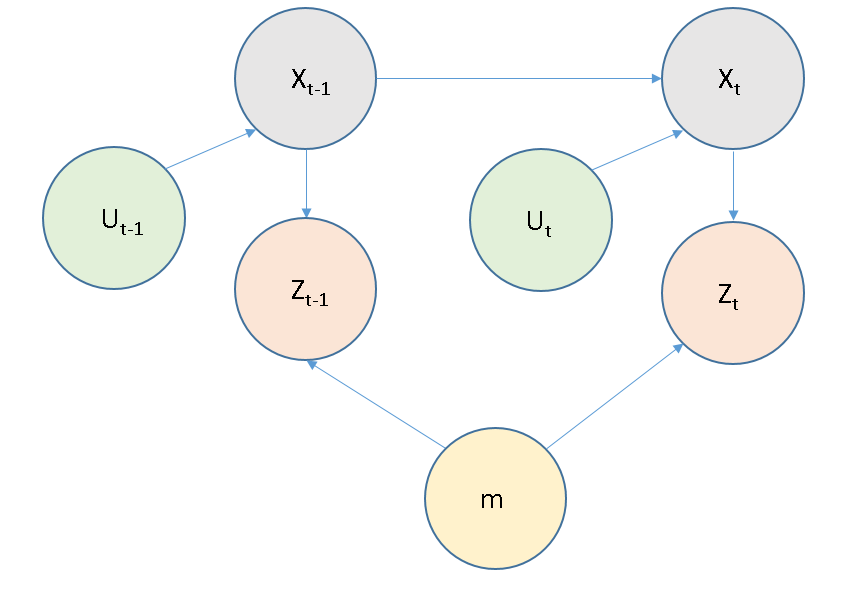
\includegraphics[width = 0.5\linewidth]{Chapters/MultiAgentTargetDetection/BayesianFiltering/Figs/DBNs/2DBNExample.png}
    \caption{A DBN used for \textbf{S}imulatenous \textbf{L}ocalisation \textbf{A}nd \textbf{M}apping (SLAM), based on \cite[p.~311]{Thrun:2005:ProbabilisticRobotics}}
    \label{fig:2TDBNExample}
\end{figure}


\subsubsection{}
\label{Chapter:DBN}

\subsection{Inference Using HMMs and DBNs}\label{subsection:InferenceHMMDBN}
As discussed, HMMs and DBNs are useful tools for modelling complex random dynamic processes. Typically, models are used to provide some kind of inference about a process, to gain insight into its inner workings. By inference, we mean calculating the probability distributions over variables of interest. Some algorithms will be outlined here that will demonstrate how to calculate both exact and approximate inferences, using general structures for HMMs and DBNs. \par

First HMMs are discussed, as their representation more rigid, meaning that it is easier to exploit their structure generally to perform inference. The first and arguably most useful quantity that we want to compute is 
\[P(X_t | e_{1:t})\]
that is, the probability distribution of the hidden state variable, given all previously observed evidence variables. This is the \textit{filtering} problem, mentioned in section \ref{Chapter:HMM}. We are interested in computing this value, rather than the unconditional state distribution, $P(X_t)$, because .... The conditional distribution $P(X_t | e_{1:t})$ is frequently referred to as the \textit{belief state} and the process of calculation of this distribution is frequently referred to as \textit{state estimation} or \textit{filtering}. The \textit{forward algorithm} is frequently used to calculate the value of $P(X_t | e_{1:t})$. It is a recursive algorithm, and takes advantage of the fact that the underlying process is Markovian. The well-known forward algorithm for HMMs is shown in algorithm \ref{algo:bayes_filter_observations_only}. 

%\begin{algorithm}
%\SetAlgoLined
%\KwResult{Write here the result }
% initialization\;
% \While{While condition}{
%  instructions\;
%  \eIf{condition}{
%   instructions1\;
%   instructions2\;
%   }{
%   instructions3\;
%  }
% }
 
%\end{algorithm}

\begin{algorithm}
\caption{Generating the RAV Agent Routes}
\label{alg:bayes_filter_observations_only}
\begin{algorithmic}[1]
\renewcommand{\algorithmicrequire}{\textbf{Input:}}
\renewcommand{\algorithmicensure}{\textbf{Output:}}
\REQUIRE Array of agents, Set of coordinates, Cost function which takes two GPS coordinates and outputs a real number representing the cost of travelling from one to the other. 
\ENSURE  A key-value container of agents and their corresponding routes.\\
\hfill\pagebreak

\noindent\textbf{\textit{\noindent Initialization} :}\\
agentPaths$\leftarrow$empty key-value container\\
visitedPoints$\leftarrow$empty array
\\
For each agent in agents:\\
\quad Initialise path of agent as empty array in agentPaths
currentAgentIndex$\leftarrow$0\\
currentAgent$\leftarrow$agents.get(currentAgentIndex)\\
\hfill\pagebreak

\WHILE {pointsToVisit is not empty}

\STATE agentPosition $\leftarrow$ last value in agentPaths.get(agent)

\STATE P$\leftarrow$\(\displaystyle \min_{p \in pointsToVisit}\)cost(agentPosition, p)

\STATE Update currentAgent value in AgentPaths to include P
\STATE Add P to visitedPoints.
\STATE Remove P from pointsToVisit.
\STATE currentAgentIndex$\leftarrow$(currentAgentIndex+1) $\mathbf{mod}$$\vert$List of Agents$\vert$
\STATE currentAgent$\leftarrow$agents.get(currentAgentIndex)


\ENDWHILE
\RETURN agentRouteMap
\end{algorithmic} 
\end{algorithm}

\note{Don't forget to mention: Sufficient statistics, forward algorithm}




\subsection{Prediction Algorithms}
\placeholder{}
This contains the details of prediction algorithms
%%%%%%%%%%%%%%%%%%%%%%%%%% Bayesian Filtering Sections %%%%%%%%%%%%%%%%%%%%%%%%%%



\section{Methodology}

\note{Want to outline the process by which the problem was solved in some kind of logical manner. Current idea for structure: }
\note{First identify the problems that ROCSAFE presents}
\note{Instead of rushing headlong into solving difficult problem, identify key aspects of harder problems and develop a suitable method of solving that, making simplifying assumptions as necessary}
\note{Created test-bed in order to explore and evaluate possible solutions}
\note{Identified DBN as a suitable tool to model the problem with flexibility to extend to more complex verions}
\note{Then discuss how DBN and corresponding algos/strategies were modified to incorporate multiple targets, battery and other agents.}

%Contains the restructured agent design etc.

\chapter{Multi-Agent Stochastic Target Localization}\label{chap:targetLocalisation}
\workinprogress
This chapter outlines the approach taken to solve the research question stated in the introduction chapter. The context for this problem is derived from the ROCSAFE project \cite{rocsafeNUIG}. \note{Not sure how best to present the problem and how to provide the necessary content to naturally leads to the approaches discussed here. Fill this out further once research questions have been finalized/refined}


\section{Problem Description}\label{sec:TLocalisationProbDescription}
As mentioned in Chapter \ref{chapter:introduction}, a major problem in hazardous scene management includes localizing sources of hazardous materials and localizing potential sources of evidence. The reasons these are difficult problems, in the context of the ROCSAFE project, are:
\begin{itemize}
    \item Hazardous materials belong to different classes of threat (chemical, biological, radiation, nuclear). If the nature of the threat is uncertain, the wrong preventative measures may be taken and personnel may be put at risk. 
    \item Evidence localisation usually requires moving a sensor to within close proximity of the evidence. If a human is responsible for this, there is a chance that they will accidentally disturb with the evidence, possibly yielding it unusable.
    \item Since these scenarios are highly dangerous, the area to search may be large to avoid potentially missing important sources of evidences. This means that the process of localisation may be painstaking and time-consuming for humans.
\end{itemize}
In the ROCSAFE project, the use of RAVs is proposed to aid the execution of these tasks \cite{Bagherzadeh2017ROCSAFE:Incidents}. This chapter proposes a system to aid their navigation planning.

  
%This section proposes a system that can aid the execution of these tasks using a system of automated \textbf{U}nmanned \textbf{A}erial \textbf{V}ehicles (RAVs). \par



Spatiotemporal localisation problems have a reasonable body of literature behind them, and can be described using abstract language which allows them to be approached using a common framework, with only minor implementation details necessary to specify which instance of the problem is being addressed. The framework we have developed uses a lot of the theory outlined in Chapter \ref{chapter:Background} and builds on the literature that was reviewed there. The problem that this Chapter attempts to solve can be generally described as follows: \par

\textit{Given a region of space to explore and a set of heterogeneous autonomous aerial vehicles with sensing capabilities, devise a search strategy with a search cutoff criterion which will accurately return either the locations of the targets if one or more is present, or return that no targets are present, in the shortest possible time.} \par

We designed the system to be general, but we list some concrete versions of this problem that we envisage this approach could effectively solve:
\begin{itemize}
    \item \textit{Given a system of heterogeneous autonomous aerial vehicles, some of which are equipped with radiation sensors and limited battery capacity, localize multiple sources of radioactive material in a scene.}
    \item \textit{Given a system of heterogeneous autonomous aerial vehicles, some of which are equipped with high-quality cameras and limited battery capacity, localize multiple objects of a given description in a scene.}
\end{itemize}
Note that we do not give the details of how to solve these specific instances of the problem.
%not sure whether I should mentioned about battery etc. here or to let the discussion lead to this naturally.
\par
%In order to solve this problem, we took an approach suggested by previous works in the literature \cite{PollockSearchInterfaces} <add more here>, which break down the localisation problem into phases, between which we consider interfaces that allow the composition of various methodologies to be applied. The literature review behind this is outlined in section <reference the section>.


%\note{Did not attempt to solve this full problem in one go, instead took a simplified version and then gradually added in constraints.}

\subsection{Initial Assumptions}
\note{may need to rename this. want to convey that initially, we made some simplifying assumptions that isolate key aspects of problem that need to be solved. Then these assumptions were modified to deal with the more complex problem involving battery etc.}

Rather than immediately attempting to tackle the full problem, we chose to initially make some simplifications in order to identify potential solution strategies that could be extended to more complex versions of the problem. At the outset, we made the following simplifying assumptions:
%As outlined in the literature review, this problem has been approached before by treating the problem as a 2 Time Slice Dynamic Bayesian Network (2TDBN). 
\begin{itemize}
    \item There are either zero or one targets to be localized.
    \item The UAVs have unlimited battery capacity.
    \item The region that the UAVs need to search can be well approximated by a polygon.
    \item The sensor specificity and sensitivity are known or can be estimated for a given resolution (e.g. 1m). These are assumed to be greater than 50\% for the given resolution.
    \item The UAVs operate over a discrete spatial grid spanning the region to search, assumed to be polygonal as above, the dimensions of which are pre-determined by the sensor resolution.
    \item The UAVs are assumed to have a GPS sensor that is accurate to beyond the sensor resolution (implying that the UAV moves to discrete grid locations without drift).
    \item The target is assumed to be small enough to occupy only one grid cell at a time. It is also assumed to not lie across grid cells.
\end{itemize}
While these assumptions are clearly unrealistic, they are convenient because they simplify the design of the system and subsequent analysis. In later sections in this chapter, these assumptions are relaxed and the necessary modifications for the solution strategy are discussed. Some ramifications of these assumptions are addressed later in the chapter, at section <x>. It is worth noting that similar simplifying assumptions were made in related works in the literature, 
(\cite{Chung2007ASearch} and \cite{Waharte2010SupportingUAVs}), % find additional citations in mendeley
which strongly influenced our initial approach.

\subsection{Experimental Testbed}
Given the assumptions outlined above, rather than beginning by working on designing candidate solutions, we instead decided to set up the software that would be necessary to quickly test and evaluate a solution. This is related to the specification of the agent's environment, which is described in subsection \ref{subsection:intial_agent_design}. This involved the following software components:
\begin{itemize}
    \item A 2-Dimensional grid coordinate system which can be easily configured to create a grid over a polygonal region. This is outlined in greater detail in section <provide a reference to the section>.
    \item An evidence source simulator which simulates the readings that a sensor would observe given the sensitivity and specificity of the sensor.
    \item A grid manager component, which manages the positions of RAVs and targets on the grid.
    \item A simulation manager component, which constructs the agents from their configuration files and is responsible for running the simulation using the other software components.
    \item Configuration files which allow the user to specify the configurations of the sensors, the agents, environment parameters and debugging/analysis files.
\end{itemize}
These components were designed in a modular fashion to distinguish the agent from its environment, shown in Figure \ref{fig:agent_env_interaction}. This seems like an obvious and intuitive practice, but can be easily overlooked while writing code. For example, the agent may have an internal representation of the grid environment in which it operates which should be completely independent of the actual grid environment which is run in the simulation. The user can fully specify all aspects of the agent and environment (relating to the above assumptions) through configuration files. \note{Maybe include an example figure showing a config file.}



%This file contains all the details of agent design using files in initialAgentDesign folder




\section{Agent Design}\label{section:intial_agent_design}
\note{addressed some of these simultaneously (i.e. once I had decided model-based agent, then had to answer question of what model will look like)}
\note{probably best to list these individually with some corresponding discussion}

When designing the agent, we adhered the approach outlined in Chapter 2 of "\textit{Artificial Intelligence: A Modern Approach}" \cite{AIAMA}. First, we describe four critical parts of the agent design, collectively referred to as the agent's \textit{task environment}: the Actuators, Sensors, Environment, and Performance Element. Further discussion on specific aspects of how the agent function was implemented is then given.
%where the larger multi-faceted problem is broken down into smaller individual sub-problems. 

\subsection{Agent Environment}
\note{Use of italics may not be necessary here}
\note{Should refer to previous works more here}
Here, we refer to conventional terms used to describe agent environments, described in \cite[p.~41]{AIAMA}. The agent's environment is \textit{partially observable}, since it is assumed that it cannot directly observe the location of the target, but must instead use partial information related to the location of the target from noisy sensors. The outcomes of the agent's actions are assumed to be \textit{deterministic}, meaning that if an agent chooses to move to a location, it is assumed to do so without any chance of it accidentally moving to an alternative location. The environment is \textit{sequential}, arising from the fact that future decisions on where the agent should take a sensor reading are influenced by previous locations at which a sensor reading has been taken. The agent is assumed to operate in a 2-dimensional environment, consisting of discrete uniformly spaced grid cells overlaid onto a physical region of space.
%The environment state can then defined by the tuples of the unknown location of the target with the search status.
The unknown location of the target can be described by the set
\[\{x_1, x_2, ..., x_n, x_{n+1}\}\]
where $x_i$ represents the target location being at grid cell $i$ for $i \in \{1, 2, .., n\}$, and $x_{n+1}$ represents that the target is not present. The search status can be described by 
\[ \{ongoing, terminated\_x_1, terminated\_x_2, ..., terminated\_x_n, terminated\_x_{n+1}\} \]
where $ongoing$ represents that the search is continuing and $terminated\_x_i$ is an absorbing terminal state that arises from the agent taking a terminal action indicating the target location, explained further in the subsequent paragraph. It is necessary to include the terminal states in the environment representation in order to specify a \textit{performance measure} for the agent. 
%For technical reasons, the agent's location was also included in the environment state.
The Cartesian product of these sets defines the environment state. For example, the environment might start in state $<x_3, ongoing>$, which represents that a target is located at grid cell 3 and the search is ongoing. $<x_3, terminated\_x_5$ represents that the search has terminated with the agent concluding the target is present at grid cell 5, with the target actually present at grid cell 3. The graphical model shown in Figure \ref{fig:FirstDBNUsed} depicts the conditional independence assumptions made between the hidden state variables, which is explained in Section \ref{subsec:stochasticEnvModel}.
%\note{Goal state not explicitly mentioned - might be worth explicitly stating.}

\subsubsection{Actuators and Sensors}
Here we consider the actions that may be chosen to be performed by actuators and percepts that may be received by sensors. The problem of \textit{target localization} in the context of this chapter requires the agent to move around a discrete grid and use a calibrated sensor to record noisy readings that indicate whether the target is present or not at the location of the reading. It is therefore intuitive to describe the set of possible actions to be performed by the actuators by the set of all $n$ possible grid locations that the agent can move to and take a sensor reading at, indexed by an arbitrary ordering: $\{move\_x_1, move\_x_2, ..., move\_x_n\}$. We add additional actions to this set, $\{terminate\_search\_x_{i}\}$, for $i \in \{1, 2, ..., n, n+1\}$, which lead to an absorbing terminal state representing the agent's conclusion regarding whether a target is present or not, $terminated\_x_{i}$ . The set of percepts that the agent will receive from its sensors come from the binary set \{1, 0\}, indicating the target has or has not been detected, respectively.

\subsection{Performance Measure}\label{sssection:PerfMeas}
The agent's performance measure maps sequences of environment states to the real numbers. Given the above definitions, we decided that environment states of the form
\[ <x_i, terminated\_x_i> \]
should be of high value, as they indicate that the agent has correctly identified the location of the target in the environment. Secondary to this, sequences of environment states that take longer to end in a terminal state should be valued lower than shorter ones, reflecting our desire for the agent to terminate its search in the minimum possible amount of time. Therefore, the performance measure primarily gives high values to the agent when it correctly identifies the location of the target or correctly concludes that the target is not present, with a secondary ordering on value determined by the time taken to come to a conclusion. The actual value of the function only needs to adhere to this ordering, but arbitrarily defined it as:
%\note{Be careful that this agrees with the rest}
\[
Performance Measure(state_1,..., state_t) = 
\begin{cases}
\frac{1}{t} \quad \text{ if } state_t \text{ = } <x_i, terminated\_x_i>
%agent returns correct target location.} 
\\
-1 \quad \text { otherwise. }
\end{cases}
\]

%\[
%Performance Measure(state_1,..., state_t) = 
%\begin{cases}
%\frac{1}{t} \quad \text{ if } state_t \text{ = } <x_i, TERMINATED\_x_i>
%agent returns correct target location.} 
%\\
%\frac{1}{t} \quad \text{ if agent correctly returns target is not present.}
%\\
%-1 \quad \text { if agent returns incorrect target location.}
%\\
%-1 \quad \text{if agent incorrectly returns target is not present}
%\end{cases}
%\]

%The performance measure is assumed to ignore subsequent terminal states. 
It is worth noting that this performance measure provides goal states for the agent:
\[ <x_i, terminated\_x_i> \]



\subsection{Stochastic Environment Model}
\workinprogress
Model-based agents require a concrete implementation of a model of their world, in order to maintain their internal state. The agent's internal state can be thought of as its opinion of what state the world might be in, and its model describes how it believes the world changes over time. Chapter \ref{chapter:Background} outlines the background behind potential models of the stochastic world, including both how internal state can be represented and how internal state can be updated.\par
Hidden Markov Models and Dynamic Bayesian Networks were identified as highly suitable models, due to the fact that they provide a succinct and flexible representation of hidden stochastic world state, as well as efficient online state estimation updating algorithms. We chose to use a Dynamic Bayesian Network (DBN), due to the fact that it can help overcome some of the limitations that HMMs potentially may present (outlined in chapter \ref{chapter:Background}). DBNs also facilitate the incorporation of extra variables with arbitrary conditional dependence relations. This was desirable, since we planned to extend the model to include extra variables, such as battery level, once a basic implementation was shown to work as intended.

The 2-Time Slice DBN used is shown in figure \ref{fig:FirstDBNUsed} describes the agent's world model. A first-order Markov assumption is made, where the current state only depends on the state directly preceding it. Grey coloured variables are \textit{hidden state variables} and are assumed to not be directly observable. Green coloured variables are \textit{control actions} taken by the agent (which use the agent's estimated state) and the peach coloured variables are \textit{evidence variables}, which are assumed to be observable and depend on the hidden world state. 
%The agent's location and the search status hidden state variables are mainly included for technical reasons
\note{maybe re-position figure so text wraps}
\begin{figure}
    \centering
    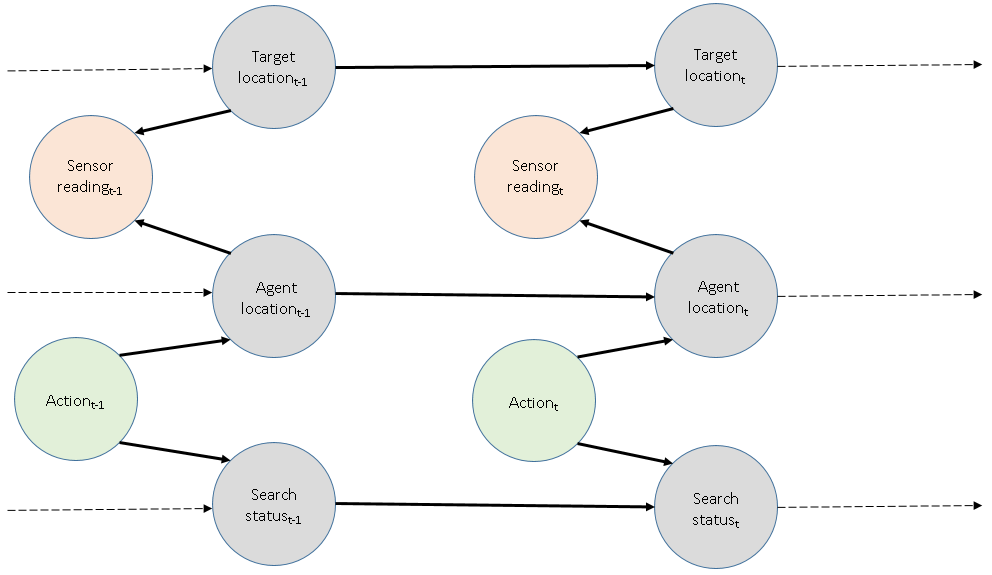
\includegraphics[width = 0.8\linewidth]{Chapters/MultiAgentTargetDetection/Figs/DBNWithMultipleHiddenState.PNG}
     \caption{First Version of the DBN representing the agent world model}
    \label{fig:FirstDBNUsed}
\end{figure}
A number of conditional probabilities are specified here in order to describe the factored joint distribution of the world model fully. The full tables are omitted as they are sparse. For brevity, we use the abbreviation Loc for Location.



\begin{figure}[H]
\scriptsize
\begin{equation}\label{eqn:EvidenceVarsProbs}
    %\centering
    p(SensorReading_t | AgentLoc_{t-1}, EvidenceLoc_{t-1})  = 
    \begin{cases}
    \alpha \quad \text{ if } SensorReading_t=1 \text{ and } EvidenceLoc_t \neq AgentLoc_t
    \\
    1-\beta \quad \text{ if } SensorReading_t=1 \text{ and } EvidenceLoc_t = AgentLoc_t
    \\
    \beta \quad \text{ if } SensorReading_t=0 \text{ and } EvidenceLoc_t \neq AgentLoc_t
    \\
    1-\alpha \quad \text{ if } SensorReading_t=0 \text{ and } EvidenceLoc_t \neq AgentLoc_t
    \end{cases}
    %
\end{equation}
\caption{Conditional Probability Distribution for the $Evidence$ Variable}
\end{figure}


\begin{figure}[H]
\scriptsize
\begin{equation}\label{eqn:TargetLocProbs}
    p(TargetLoc_{t} | TargetLoc_{t-1}) =
    \begin{cases}
    1 \quad \text{ if } TargetLoc_{t}=TargetLoc_{t-1}
    %agent returns correct target Loc.} 
    \\
    0 \quad \text { otherwise. }
    \end{cases}
\end{equation}
\caption{Conditional Probability Distribution for the $TargetLocation$ Variable}
\end{figure}





\begin{figure}[H]
\scriptsize
%\begin{equation}\label{eqn:SearchStatus}
    \begin{gather}\label{eqn:SearchStatus}
        p(SearchStatus_t | SearchStatus_{t-1}, Action_{t-1}) = \\
        \begin{cases}
        1 \quad \text{ if } SearchStatus_t = terminated\_x_i \text{ and } SearchStatus_{t-1} = terminated\_x_i 
        \\
        1 \quad \text{ if } Action_t = terminate\_x_i \text{ and } SearchStatus_{t-1}=ongoing \text{ and } SearchStatus_{t} = terminated\_x_i
        \\
        1 \quad \text{ if } Action_t = move\_x_i \text{ and } SearchStatus_{t-1}=ongoing \text{ and } SearchStatus_t=ongoing
        %agent returns correct target location.} 
        \\
        0 \quad \text { otherwise. }
        \end{cases}
    \end{gather}
%\end{equation}
\caption{Conditional Probability Distribution for the $SearchStatus$ Variable}
\end{figure}





\begin{figure}[H]
\scriptsize
    \begin{equation}\label{eqn:AgentLocation}
        p(AgentLoc_t | AgentLoc_{t-1}, Action_{t}) = 
        \begin{cases}
        1 \quad \text{ if } Action_t = move\_x_i \text{ and } AgentLoc_t = x_i
        \\
        1 \quad \text{ if } Action_t = terminate\_x_i \text{ and } AgentLoc_t = AgentLoc_{t-1}
        \\
        0 \quad \text{otherwise}
        \end{cases}
    \end{equation}
\caption{Conditional Probability Distribution for the $AgentLocation$ Variable}
\end{figure}


\normalsize
The semantics of the equations listed above is given here: 
\begin{enumerate}
    \item Equation \ref{eqn:EvidenceVarsProbs} uses two parameters, $\alpha$ and $\beta$, to represent the probability of making a false positive and false negative sensor reading, respectively. These are assumed to have been calculated by using pre-calibrated values of the sensor. This model is very flexible and does not stipulate any restrictions on the sensor other than that it must return a reading indicating that the target is present or not.
    \item  Equation \ref{eqn:TargetLocProbs} simply states that the location of the target does not change, even though it is hidden. It would be very easy to modify this to allow for moving target detection in the case of a non-static target.
    \item Equate \ref{eqn:SearchStatus} is also states a number of intuitive notions. The first line states that once the agent terminates the search, it remains over. The second line states that if the agent requests an ongoing search to terminate, then it does so deterministically. The third line states that if the agent chooses to move in an ongoing search, then the search remains ongoing.
    \item Equation \ref{eqn:AgentLocation} simply outlines that the agent moves to new locations deteministically. It also indicates that should the agent choose to terminate the search, then the environment enters a terminal state, indicating that the search is over.
\end{enumerate}


Note that despite the fact that some hidden state variables cannot be observed directly, it is still possible to infer their value exactly based on their starting state. For example, the position of the agent is a deterministic function of its actions and previous position. These variables could have been treated as variables that are internal to the agent rather than part of the hidden world state and many authors omit such variables for the sake of clarity.
\note{need to outline why I have included them - mainly because evidence probability depends on agent location as well as source location}


\subsubsection{Estimated State}
\workinprogress
Since the agent operates in a partially observable environment, the agent's internal state representation of the environment needs to take into account the fact that the current environment state is not certain. For this reason, a probability distribution over possible environment states is used by the agent to internally represent the environment state. The internal agent state is described mathematically by 
\[p(x_t | e_{1:t}, u_{1:t})\]
, which is the distribution of possible world states given all evidence and control actions up to the current time step, where $x_t$, $e_t$ and $u_t$ follow the conventions of being the hidden state variables, the evidence variables and the control action variables. The agent updates this state using the world model specified in the preceding chapter, using the filtering algorithm explained in section \ref{subsection:InferenceHMMDBN} of Chapter \ref{chapter:Background}. There are a couple of noteworthy points:
\begin{itemize}
    \item A distribution that has a single sharp peak would indicate that the agent believes that the target is at a specific location with high confidence. This is clearly preferred to a flat, uniform distribution representing uncertainty in relation to where the target might be.
    \item The only true source of uncertainty in the world state is introduced by the sensor. Therefore, analysis of this state representation in relation to the sensor model should provide insight into how the system performs.
\end{itemize}
In order to update the estimated state of the agent, the below equations are used, which are described in subsection \ref{subsection:InferenceHMMDBN}. For brevity $x_t$ denotes the hidden state variables, $e_t$ denotes the evidence variable and $u_t$ denotes the control action taken by the agent. The equations only describe the estimated state update for move actions, since if the agent terminates the search a terminal state is deterministically entered. The $SearchStatus$ variable is omitted from the equations since it only effects the equations if the $Action$ variable is to terminate the search.
\footnotesize
\begin{figure}[H]
\scriptsize
%\begin{equation}\label{eqn:SearchStatus}
    \begin{gather}\label{eqn:SearchStatus}
        p(AgentLoc_t = x, TargetLoc_t = y | e_{1:t}, u_{1:t}) = \\
        \begin{cases}
            \eta \alpha p(AgentLoc_{t-1} = x, TargetLoc_t = y | e_{1:t-1}, u_{1:t-1}) \text{ if $e_t$ is a positive reading and $AgentLoc_t \neq TargetLoc_t$} \\
            \eta \beta p(X_{t-1}=x_t | e_{1:t-1}, u_{1:t-1}) \text{ if $e_t$ is a negative reading and $Agent_loc_t$ = $TargetLoc_t$} \\
            \eta (1-\alpha) p(X_{t-1}=x_t | e_{1:t-1}, u_{1:t-1}) \text{ if $e_t$ is a negative reading and $Agent_loc_t \neq TargetLoc_t$} \\
            \eta (1-\beta) p(X_{t-1}=x_t | e_{1:t-1}, u_{1:t-1}) \text{ if $e_t$ is a positive reading and $Agent_loc_t$ = $TargetLoc_t$} \\
        \end{cases}
%\eta O_{t} T^{T} f_{1:t-1} 
    \end{gather}
\end{figure}
\normalsize


\subsection{Action Selection Strategies}\label{subsubsec:ActionSelection}
At each discrete time step the agent may either choose to terminate the search or move to a new location to take a measurement reading. The agent may choose which of these actions to perform based on its location, the search status and its internal representation of the environment, which are outlined in the preceding section. First we discuss how move actions are chosen, if the agent decides that the search should not be terminated at the current time step. We began by implementing some of the recommended basic search strategies outlined in the related works by \citeauthor{Chung2007ASearch} \cite{Chung2007ASearch} and \citeauthor{Waharte2010SupportingUAVs} \cite{Waharte2010SupportingUAVs}. These search methods are devised in order to optimize the agent's performance measure, which is set out in Section \ref{sssection:PerfMeas}. The results of applying these strategies are discussed in Section \ref{sec:SimulationResults}.\par 
%\note{In the following, might be good to mention the motivation in relation to the performance measure}
\textbf{Random Search}
This method serves as a baseline against which similar strategies can be compared. The agent simply chooses the next grid location to explore randomly from all possible grid locations. The expected number of moves needed to take a reading at all possible grid cells is given by the solution to the \textit{coupon collectors problem} \cite{Erdos1961OnTheory}, $nH_n$, where $H_n$ is the $n_{th}$ harmonic number and $n$ is the total number of grid cells, which gives a good idea of the expected amount of time that will be taken to conclude the search.

\textbf{$\epsilon$-Greedy Search}
A simple greedy search was implemented next, where the agent chooses to visit the grid cell with the highest estimated probability of containing the target in a localized region around the agent:
\footnotesize
\[
Action_t = \argmax_{NewLoc \in N(AgentLoc)}{p(TargetLoc = NewLoc, SearchStatus, AgentLocation| e_{1:t}, u_{1:t})}
\]
\normalsize
$N(AgentLoc)$ is a function that returns a neighborhood of locations around the agent's location and can be calibrated to trade off the cost of saccading between grid cells that may be far from each other against the cost of limiting the agents range to a narrow and possibly "cold" region.This method is designed bearing in mind that there may be motivation to explore some areas before others based on prior knowledge. 

%\textbf{$\epsilon$-greedy Search} Greedy search  simplest method to implement was an $\epsilon$-greedy action selection method, whereby the agent moves to the grid cell with the highest estimated probability in a pre-defined radius with probability 1-$\epsilon$ and a random grid cell in the pre-defined with probability $\epsilon$. This encourages the agent to exploit it's current know\par

\textbf{Saccadic Search}
This was proposed in \cite{Chung2007ASearch} and is a special case of $\epsilon$-greedy search. The idea is to mimic the behaviour of the human eye when looking at an image, whereby it "\textit{saccades}" from one salient feature to another. The consequence is that the most promising cells are explored at each time step, which means that the agent can be drawn to travel large distances in order to explore a peak in the spatial distribution given by the occupancy grid. Further details are given in \cite{Chung2007ASearch}.

\textbf{Sweep Search}
This strategy sweeps the region of interest systematically, aiming to take a reading at each grid cell an equal number of times while minimizing the total distance travelled. It then traverses this same path again in reverse order. This requires planning a trajectory in advance, which is often referred to in related literature as the \textit{complete coverage path}. Since the region to be swept is assumed to be a grid, where adjacent points are assumed to be equidistant, a number of heuristic solutions were available for use from Section \ref{sec:SceneSurveying}.\par

%\textbf{POMDP Based Search} 
%\note{Not sure if I should go into this at all. Work was done in understanding POMDPs and clearly the solution can be easily framed as a POMDP but my work stopped short in actually finding a solution to POMDP that works well}
%As outlined in 
%details. \par


\subsection{Search Termination}\label{subsubsec:SeachTerminationMethodology}

At each discrete timestep, the agent can either choose to move to a new grid location to record a sensor measurement or it can decide to terminate the search based on its estimated state of the environment. There is a trade-off in terminating the search early, which means that less time and resources are spent on continuing the search, versus the possibility of drawing misinformed conclusions from the search due to a lack of information. For example, if the agent receives a series of false positive readings at a given location, it could mistakenly choose to conclude that the target is present at a given location rather than sample further to gain confidence that it has correctly found the location of the target. Following this line of thinking, it is clear that a strategy needs to be devised to minimize the probability of drawing false conclusions, which is described in the performance measure set out in Section \ref{sssection:PerfMeas}.\par
\citeauthor{Pollock1971SearchInterfaces} outlines three commonly used criteria that can be used to make a decision whether to terminate the search or not: the \textit{Bayes Criterion}, which minimizes the expected cost per decision, the \textit{Minimax Criterion}, which chooses a decision which minimises the maximum expected cost and the \textit{Neyman-Pearson Criterion}, which uses a likelihood ratio test to determine the optimal decision to make \cite{Pollock1971SearchInterfaces}. These tests are proposed in the context of a target that is definitely present in the search region, but can be extended to incorporate the decision problem where the target may or may not be present. In addition, related work by \citeauthor{Chung2007ASearch} has addressed this problem using methods that use heuristics to make a decision whether to terminate the search or not \cite{Chung2007ASearch}. 

We ultimately choose to implement the Sequential Probability Ratio Test (SPRT), which is a hypothesis-testing framework developed by \citeauthor{Wald1950BayesProblems} to optimally deal with sequential decision problems, as opposed to traditional frameworks which assume that all the necessary data has been gathered prior to analysis \cite{Wald1950BayesProblems}. The background knowledge behind the SPRT can be found in Section \ref{subsec:SPRT}. An algorithm is also provided on how to perform this test in practice.
%The details of the proof of optimality of the SPRT is given in \cite{Wald1950BayesProblems} and we have outlined the details of how to perform hypothesis-testing using this framework in section <refer to the section>, along with the practical advantages and drawbacks of using it. 
We applied the SPRT algorithm to our problem to provide a search termination criteria using the following quantities: 
%In order to allow the agent to make a decision on whether to terminate the search or not, the following procedure was used: \note{Might be worthwhile simply outlining the algorithm}

\begin{gather}\label{eqn:SPRTQuantities}
H_0 : \text{The null hypothesis, the target is not present in the search region}\nonumber
\\ \nonumber
H_1 : \text{The alternative hypothesis, the target is present in the search region}\nonumber
\\ \nonumber
\alpha : \text{The maximum probability of making a type } \Romannum{1} \text{ error.} \nonumber
\\ \nonumber
\beta : \text{The maximum probability of making a type } \Romannum{2} \text{ error.}\nonumber
\\ \nonumber
\\ \nonumber
p_{0t} : \text{ The probability of observing the data $(e_1, ..., e_t)$ under the assumption of $H_0$} \nonumber
\\ \nonumber
p_{0t}=\sum_{loc=1}^{n} p(TargetLoc_t = loc, AgentLoc_t, SearchStatus_t| e_{1:t}, u_{1:t})\nonumber
\\ \nonumber
\\ \nonumber
p_{1t} : \text{ The likelihood of observing the data $(e_1, ..., e_t)$ under the assumption of $H_1$} \nonumber
\\ \nonumber
p_{1t}=p(TargetLoc_t = n+1, AgentLoc_t, SearchStatus_t | e_{1:t}, u_{1:t})\nonumber 
\end{gather}

$p_{0t}$ and $p_{1t}$ are calculated by using the evidence likelihood algorithm, which is described in detail in Section \ref{subsubsec:EvLikelihood}. The SPRT algorithm was then used at each timestep to decide whether to 
\begin{enumerate}
    \item Terminate the search accepting $H_0$, that the target is not present in the search region.
    \item Terminate the search accepting $H_1$, that the target is present in the search region. In this case, the target location with the highest estimated probability is returned as the target location.
    \item Continue the search, using the Action Selection Strategy described in Section \ref{subsubsec:ActionSelection}.
\end{enumerate}
In practice, we often took logarithmic transforms of the values used in the SPRT, to simplify some calculations and to be able to look at plots that are less heavily skewed and simpler to interpret.

\subsection{Analysis of Search Termination Criteria}
The two parameters, $\alpha$ and $\beta$ that the user needs to specify to perform the SPRT need to be chosen carefully and depend on the context of the search. As in the standard hypothesis testing context, it is important to consider the significance level and power of the test to ensure that they reflect the severity of drawing an incorrect conclusion \cite{IntroductionToMathematicalStatistics}. They can also help to perform analysis on how well the agent could perform, since setting a high threshold means that the agent may have to take a minimum number of samples at the correct target location in order to choose $H_0$ or $H_1$. \par

Figure \ref{fig:SPRTCutoffFunctionOfAlphaAndBeta} shows how A and B vary as functions of the parameters $\alpha$ and $\beta$ on a log scale
%\footnote{Tables of the values of A and B for varying for varying Type \Romannum{1} rates ($\alpha$) and Type \Romannum{2} ($\beta$) error rates may be referred to in Appendix \ref{chap:AppendixOne}.}. 
Tables of the values of A and B for varying for varying Type \Romannum{1} rates ($\alpha$) and Type \Romannum{2} ($\beta$) error rates may be referred to in Appendix \ref{chap:AppendixOne}.
If the log-likelihood ratio of the data lies in between the red and blue surfaces on the graph, another sample is taken. A projection of this plot is shown in Figure \ref{fig:VaryingSPRTParametersProjected1}:
\begin{enumerate}[label=(\alph*)]
    \item shows a plot of how varying the Type \Romannum{1} error rate $\alpha$ for a fixed Type \Romannum {2} error rate $\beta = 0.07$ affects the decision boundaries defined by A and B.
    \item shows a plot of how varying the Type \Romannum{2} error rate $\beta$ for a fixed Type \Romannum{1} error rate $\alpha = 0.1$ affects the decision boundaries defined by A and B.
\end{enumerate}

Figures \ref{fig:SPRTCutoffFunctionOfAlphaAndBeta} and \ref{fig:VaryingSPRTParametersProjected1} reflect the intuition behind the decision boundaries. The lower the probability of making either a Type \Romannum{1} or Type \Romannum{2} error, the further apart the decision boundary becomes, meaning the likelihood ratio must be very far apart from 1, which appears as 0 on the log scale. A likelihood ratio of 1 indicates maximum uncertainty. It is also possible to see that the surfaces meet when $\alpha=0.5$, $\beta=0.5$, which reflects the fact that immediately terminating the search will give a 0.5 probability of returning a false positive or false negative. \par

\note{Might be better off editing these images with explicit labels showing regions in which H0 and H1 will be accepted.}
Figure \ref{fig:VaryingSPRTParametersProjected2} shows the regions in which the SPRT will elect to take another sample (the green shaded region), to accept $H_0$, the upper red shaded region, and to accept $H_1$, the lower red shaded region. The blue line shows the log-likelihood ratio of $\frac{(e_{1:t} | H_0)}{p(e_{1:t} | H_1)}$ as a function of the agent belief that the target is present in the search region. 
\note{This is not really clear, should exaggerate this more}
Note that since the values of $\alpha$ and $\beta$ are significantly smaller in Figure \ref{fig:VaryingSPRTParametersProjected2} (b) than in Figure \ref{fig:VaryingSPRTParametersProjected2} (a), the acceptance region for $H_0$ and $H_1$ are significantly smaller in (b) than in (a).

\par
%varying the type \Romannum{1} error rate for a fixed type \Romannum{2} error rate affects the upper and lower threshold for cutting off the search. Figure \ref{fig:SPRTVaryingT2} shows how the varying the type \Romannum{2} error rate for a fixed type \Romannum{1} error rate affects the upper and lower threshold for cutting off the search. Note that as the varying error rate increases on the x-axis, the decision boundaries come closer together, reflecting the intuition that we are more willing to accept a mistaken conclusion.
%\begin{figure}
%    \centering
%    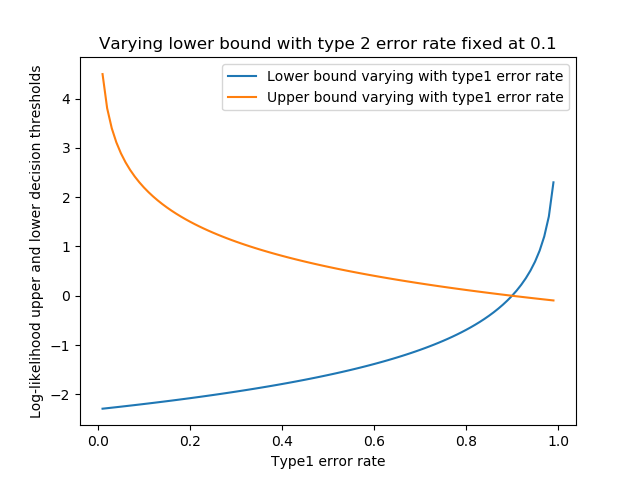
\includegraphics[width = 0.75\linewidth]{Chapters/MultiAgentTargetDetection/Figs/SearchTermination/SPRTDecisionThresholdVaryingT1ErrorRate.png}
%    \caption{The Log-likelihood upper and lower threshold for a varying type \Romannum{1} error rate and fixed type \Romannum{2} error rate.}
%    \label{fig:SPRTVaryingT1}
%\end{figure}

%\begin{figure}
%    \centering
%    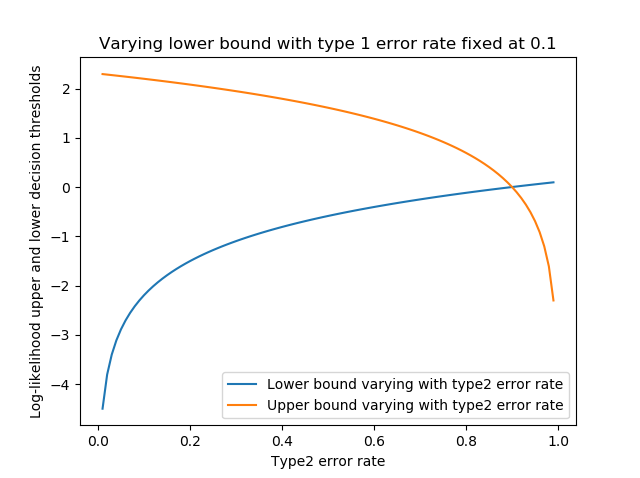
\includegraphics[width = 0.75\linewidth]{Chapters/MultiAgentTargetDetection/Figs/SearchTermination/SPRTDecisionThresholdVaryingT2ErrorRate.png}
%    \caption{The Log-likelihood upper and lower threshold for a varying type \Romannum{2} error rate and fixed type \Romannum{1} error rate.}
%    \label{fig:SPRTVaryingT2}
%\end{figure}

%Show how A and B vary for a fixed T1 or T2 error rate.
\begin{figure}[H]
    \centering
    \subfloat[Varying T\Romannum{1} error rate for a fixed T\Romannum{2} error rate]{{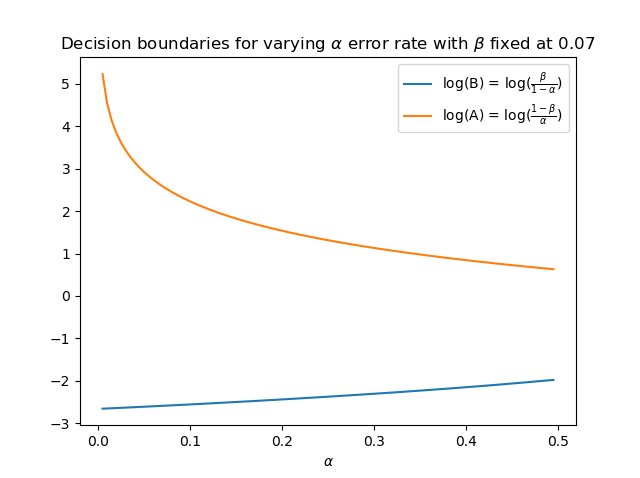
\includegraphics[width=11cm]{Chapters/MultiAgentTargetDetection/Figs/SearchTermination/AAndBVaryingWithAlpha.png} }}%
    \qquad
    \subfloat[Varying T\Romannum{2} error rate and fixed T\Romannum{1} error rate]{{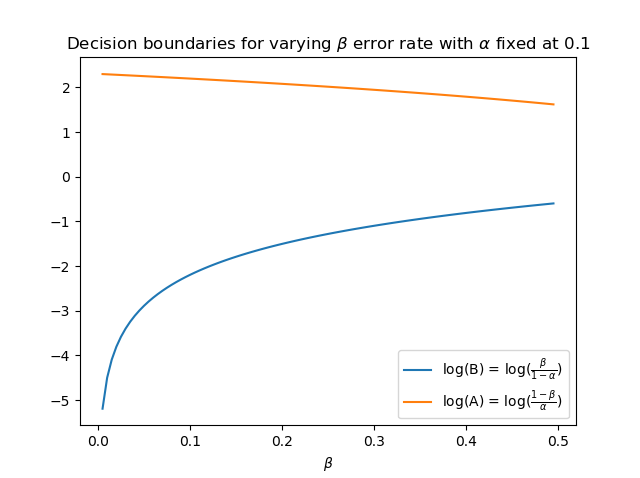
\includegraphics[width=11cm]{Chapters/MultiAgentTargetDetection/Figs/SearchTermination/AAndBVaryingWithBeta.png} }}%
    \caption{Upper and lower values of A and B for varying error rates. Values are shown on a log scale}%
    \label{fig:VaryingSPRTParametersProjected1}%
\end{figure}


%3-Dimensional plot to show how A and B vary with alpha and beta
\begin{figure}[h]
    \centering
    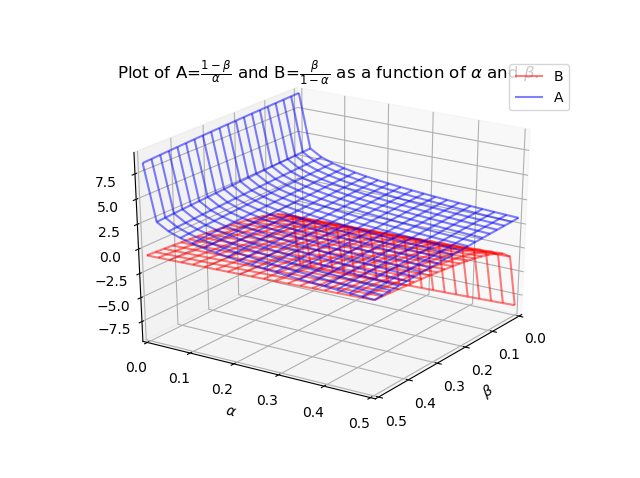
\includegraphics[width = 0.78\linewidth]{Chapters/MultiAgentTargetDetection/Figs/SearchTermination/AandBAsFunctionOfAlphaAndBetaLogTransform.png}
    \caption{The upper and lower SPRT bounds for acceptance and rejection of $H_0$, as functions of the significance and power of the test. Values are shown on a log scale.}
    \label{fig:SPRTCutoffFunctionOfAlphaAndBeta}
\end{figure}


%\begin{figure}
%    \centering
%    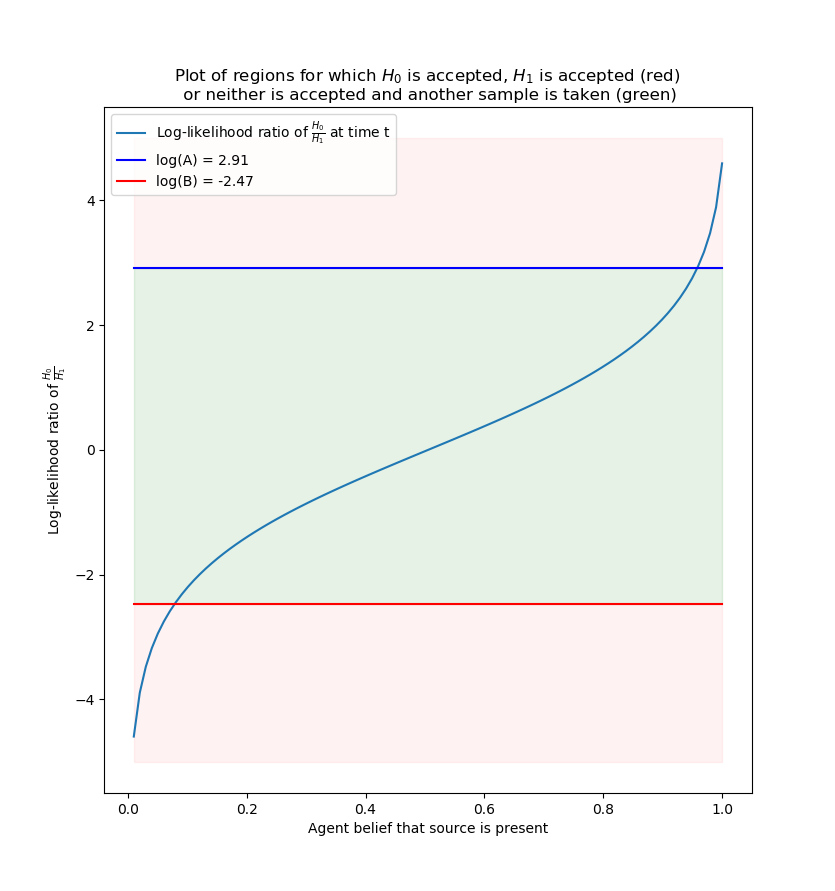
\includegraphics[width = 0.75\linewidth]{Chapters/MultiAgentTargetDetection/Figs/SearchTermination/CutoffRegions.png}
%    \caption{The cut-off regions of the SPRT for $\alpha=0.05$, $\beta=0.08$ as a function of agent belief in whether target is present or not. Values are shown on a log scale.}
%    \label{fig:SPRTLogLikelihoodRatio}
%\end{figure}

%showing how A and B create upper and lower limits for terminating the search
\begin{figure}[H]%
    \centering
    \subfloat[SPRT cut-off regions for $\alpha=0.05$, $\beta=0.08$]{{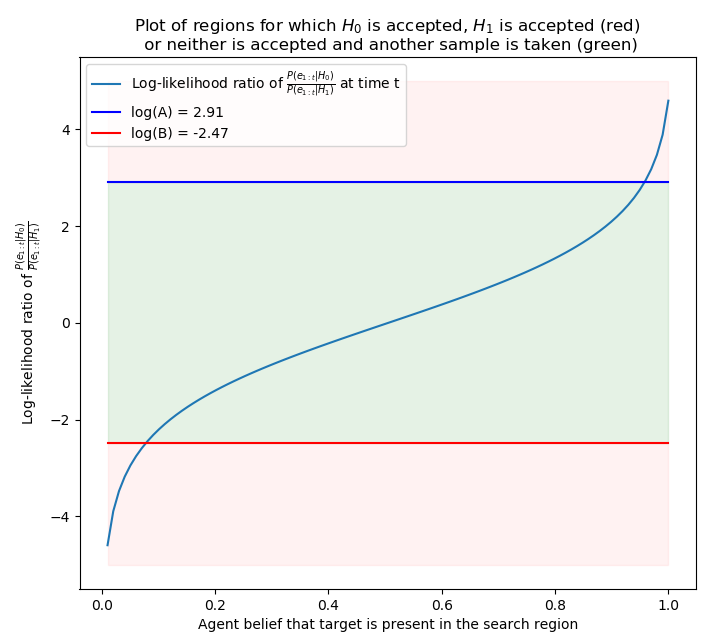
\includegraphics[width=11.5cm]{Chapters/MultiAgentTargetDetection/Figs/SearchTermination/CutoffRegionsAlphaPointZeroFiveBetaPointZeroEight.png} }}%
    \caption{} \label{fig:SPRTProjected1}
    %\qquad
\end{figure}
\begin{figure}[H]\ContinuedFloat
    \centering
    \subfloat[SPRT cut-off regions for $\alpha=0.01$, $\beta=0.02$ \label{fig:SPRTProjected2}]{{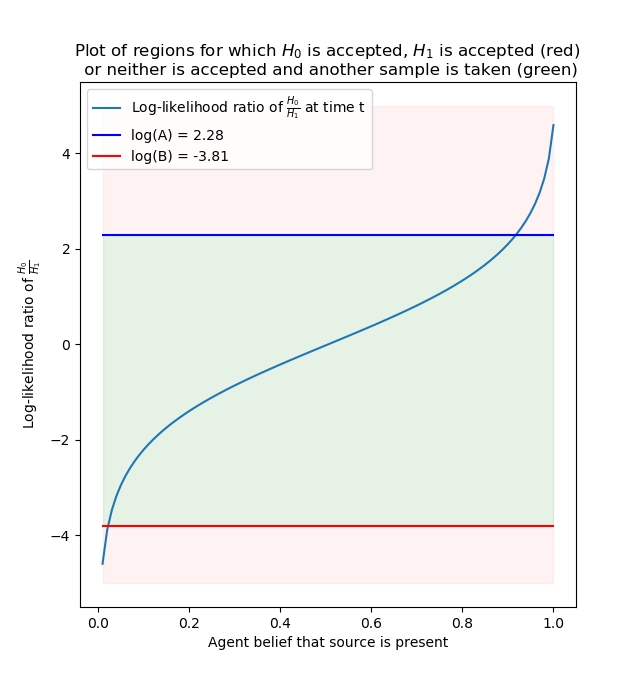
\includegraphics[width=11.5cm]{Chapters/MultiAgentTargetDetection/Figs/SearchTermination/CutoffRegionsAlphaPointOneBetaPointZeroTwo.png} }}%
    \caption{The cut-off regions of the SPRT for (a) $\alpha=0.05$, $\beta=0.08$ and (b) $\alpha=0.01$, $\beta=0.02$ as a function of agent belief in whether target is present or not. Values are shown on a log scale.}%
    \label{fig:VaryingSPRTParametersProjected2}%
\end{figure}



\note{maybe move tables to appendix}














\subsection{Agent Function Architecture}\label{subsec:AgentFNArch}
\note{This section shows how the agent function is implemented. Diagram shows how DerivedOccupancyGridAgent actually operates.}
Putting together the components outlined so far in this chapter, we end up with an agent function that is shown in Figure \ref{fig:BasicAgentArchitecture}. 

\note{Fix this figure}
\begin{figure}
    \centering
    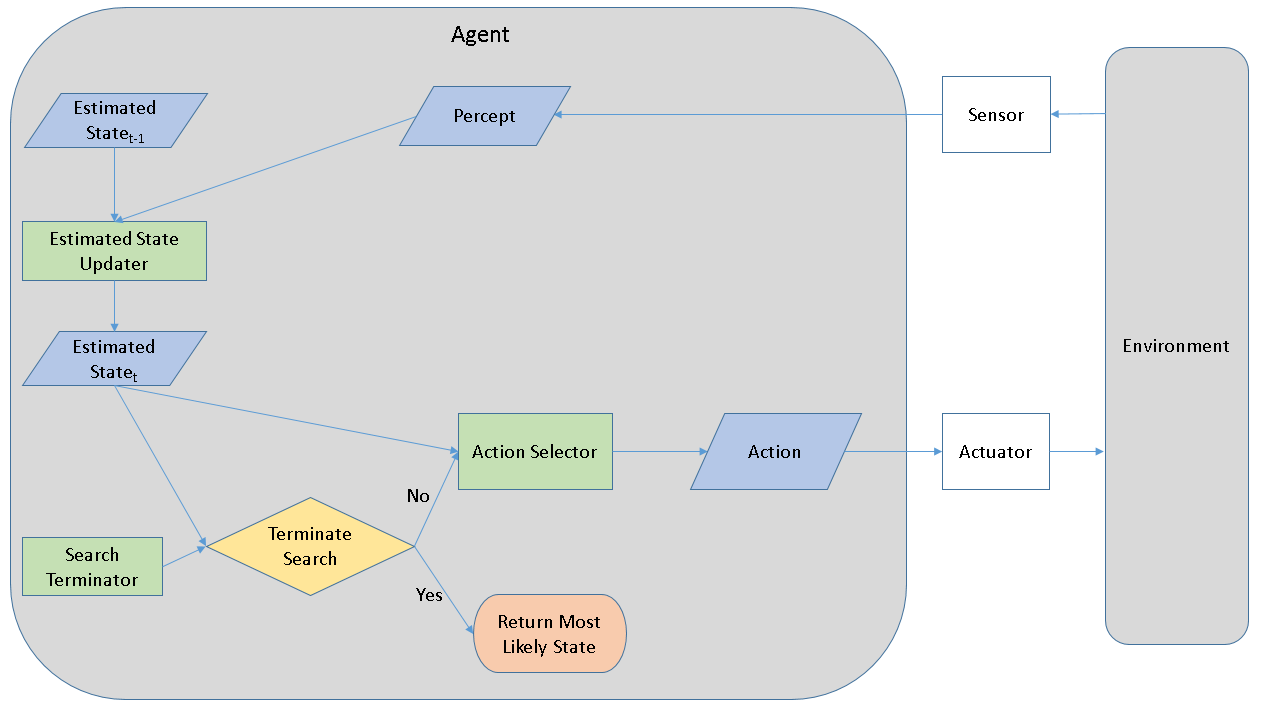
\includegraphics[width = 0.75\linewidth]{Chapters/MultiAgentTargetDetection/Figs/AgentFnArchitecture/BasicAgentFunctionNoCommunication.PNG}
    \caption{The structure of the agent function.}
    \label{fig:BasicAgentArchitecture}
\end{figure}


The diagram outlines how the agent interacts with its environment and abstracts away technical details such as the search status. This is a concrete version of the model-based reflex agent outlined in \cite[P~.51]{AIAMA}. The estimated state update rules are applied as outlined in the previous sections in this chapter. Algorithm \ref{alg:SingleTargetLocalisation} shows the algorithm which describes the agent function.
\note{might be able to bulk this up a bit, come back to it}



\begin{algorithm}{}
\caption{Single Target Localisation Algorithm}
\label{alg:SingleTargetLocalisation}

\begin{algorithmic}[1]
\renewcommand{\algorithmicrequire}{\textbf{Input:}}
\renewcommand{\algorithmicensure}{\textbf{Output:}}
%Input
\REQUIRE $ \newline initial\_estimated\_state = P(x_{0} | e_{0}, u_0), \quad \text{ The initial distribution of the estimated state}
\newline select\_action, \quad \text{Returns an action given an estimated state}
\newline estimated\_state\_updater, \quad \text{Returns the updated estimated state given the current} \newline \text{ estimated state, a percept and an action}
\newline SPRT, \quad \text{An object calibrated with a specified Type \Romannum{1}, Type \Romannum{2} error which has a method to implement} \newline \text{ the SPRT and an attribute which returns the result of the application of the SPRT.}
$
%Output
\ENSURE  $\newline \text{The grid cell containing the source, } x_i \text{ for } i \in \{1, ..., N\}, \text{ or } x_{N+1} \text{, indicating} \newline \text{ the source is not present}$

\hfill\pagebreak

\STATE $estimated\_state$ $\leftarrow$ $initial\_estimated\_state$
\WHILE{not $SPRT.should\_terminate\_search(estimated\_state)$}
\STATE $action \leftarrow select\_action(estimated\_state)$
\STATE $perform\_action(action)$
\STATE $percept \leftarrow get\_percept()$
\STATE $estimated\_state \leftarrow estimated\_state\_updater(estimated\_state, percept, action)$
\ENDWHILE
\RETURN $\argmax_{x_i}{p(x_i | e_{1:t}, u_{1:t}) = \argmax estimated\_state}$
\end{algorithmic} 
\end{algorithm}

\subsection{Extensions to the Basic Agent}
The agent design outlined in the preceding sections of this chapter addresses the problem outlined in Section \ref{subsec:ProbDescription},  following the assumptions outlined in Section \ref{subsec:initalAssumptions}. As mentioned in Section \ref{subsec:initalAssumptions}, some of these assumptions are not realistic, which we address in this section. \par

\subsubsection{Localising Multiple Targets}
The first assumption that we address is that there are either zero or one targets to be localised. In many applications, this is a very unrealistic assumption. For example, the ROCSAFE project (outlined in section \ref{sec:ROCSAFEBG}), which motivates this work, aims to apply object detection algorithms to aerial images in order to avoid the need to send a crime scene investigator into a hazardous scenario in order to verify the presence of a potential source of evidence.\note{check the above sentence is consistent with the Background} An assumption that is much more valid is that there are a maximum of $k$ unknown sources present in the search region, which addresses the general case for the ROCSAFE \note{should ROCSAFE be in italics?} project.\par

\note{May need to go into more detail here since people without a background in probability might not understand implications of high-dimensional joint distribution}
The main issue that arises when including \textit{multiple} targets in the hidden state, $X_t$, is that there is an exponential increase the dimensionality of the hidden state for each new target added. This means that maintaining an estimate of the state quickly becomes infeasible, since the run time of the forward algorithm detailed in section \ref{subsubsec:filteringDBN} is dependent on the square of the size of the joint distribution of the hidden state variables, $X_t$ and the memory requirements for maintaining the estimated state also depend on the dimensionality of the joint distribution of the hidden state. See section \ref{subsubsec:filteringDBN} for details of the filtering algorithm.


Section <reference lit review> of the literature review outlines a number of techniques that have been applied by other researchers in this domain in order to deal with the case of multiple targets. \note{maybe should leave all of this to lit. review and just outline what I did.} Related work \cite{Waharte2009CoordinatedUAVs} proposed to use an approach commonly used with occupancy grids, which is that every grid cell may or may not contain a target, independent of all other grid cells. This technique is often referred to as \textit{mapping} when the location of the agent is known. This is generally described in \cite[P.~284]{Thrun:2005:ProbabilisticRobotics}. Rather than maintain a multinomial distribution for $TargetLocation_{t-1}$, as was the case in the work outlined in this chapter, we create a new binary random variable representing a target being present or not in each grid cell, denote $m_i$ for $i \in {1,...,N}$. We denote m as the joint distribution of these random variables. 

A suitable DBN for this approach is shown in figure <>. This


In the case, estimating the joint distribution is not hard, since This results in a greatly simplified state estimate update equation, where the probability of the target being located in a grid cell does not change unless the observation was made in that grid cell. The major drawback of this approach is that there is no clear way to apply the SPRT, hence there is no clear way to decide when to terminate the search. 


stems from the fact that this assumption induces a simple dependence relation between grid cells, for which the update rule \ref{eqn:SearchStatus} can 


The first method, which is very commonly taken when using an approach that uses occupancy grids \cite{Elfes1989UsingNavigation}, is to assume that grid cells are indeped


\section{Simulation Results}

%\note{from c\&B analysis of sequential decision making}
%\note{Consider the following setting, where a single stationary tar-get is possibly located in a10×10 search region that is depicted in Fig. 5. The initial aggregate beliefB(0) is distributed among theC= 100 cells,  where  the  height  of  the  bars  in  each  cell represents the individual cell belief values, i.e., the probabilityp0cthat the target is present in a given cell, i.e.,c in {1,...,C} . SupposeB(0) = 0.75 ,  which  corresponds  to  an  initial  likeli-hood of 75\% that the target is truly present inA at the beginning of the search process. We examine the evolution of the search decision employing the different search strategies that are presented in the previous section. The search problem parameters that are used for the simulation studies, which are presented in this section, are tabu-lated in Table I. Simulations were allowed to run to completion (i.e., a decision was made), and statistics were calculated over N= 10 000 simulation replications. The values for the detec-tion errors, i.e.,alpha and beta , were chosen to reflect a representative sensor, such as a visual camera that provides aerial imagery in an outdoor and cluttered environment, which could be further calibrated empirically, e.g., by the sensor’s receiver operating characteristic (ROC) curve. Fig.  6  illustrates  the  evolution  of  the  belief  map  as  a search  agent  that  employs  the  myopic  search  strategy  thatmoves through the search region for the given search problem parameters. The searcher attempts to inspect or “clear” cells with the highest cell belief values, which, for the example bimodal belief distribution, requires visiting one peak followed by explo-ration of the other. Note that false-positive and false-negative detections  occur  throughout  the  search  process,  although  the searcher eventually arrives at the true location of the target and correctly terminates the search}


%note{From C\&B Analysis of sequential decision-making using prob. search. Consider a bounded discretized search areaA , which is de-fined byC disjoint cells. This discrete representation can charac-terize numerous environment types of diverse spatial scale, such as open areas that are relevant to maritime search operations, cluttered regions, such as obstacle-filled arenas, or structured environments, such as rooms and hallways in a building. Other factors, which include the geometry and extent of the searcher’s sensor footprint, and the size of the sought object, or other op-erational considerations (e.g., existing coordinates or reference systems) can also govern the specific cellular decomposition of the search area}

%\note{More general sensor models that account for additional spatial and/or temporal dependences be-cause  of  clutter  (indoor)  or  terrain  and  atmosphere  (outdoor) can  be  constructed  (e.g.,$\alpha$ s(k),kand $\beta$ s(k),k )  but  is  deferred for future study}


%note{In other words, the greater hindrance to deciding that a target is present in the search cell is the false-positive detection probabil-ity, since false alarms tend to prevent the searcher from “trust-ing” its positive observation. In contrast, if the missed detection probability is high, then the searcher cannot declare the search cell empty of the target with high confidence without expending multiple observations in the c}


The results presented in this section were generated by running Monte Carlo simulations of the search procedure, since finding a closed-form solution to the mean \textbf{T}ime \textbf{T}o \textbf{D}ecision (TTD) is not readily available in the general case \cite{Chung2012AnalysisStrategies}. We simulated the grid, the agents and the targets in order to evaluate the performance of the system.
%and to analyse how modifying search parameters affects the outcome.
We present statistics related to the Monte Carlo simulations, which reveal how modifying parameters of the search procedure affect the outcome. For each set of parameters in tables \ref{table:VaryingPriorDistribution}, \ref{table:VaryingInitialBelief}, \ref{table:MiscalibratedSensor}, \ref{table:MultipleTargetEGSweep}, \ref{table:MultipleTargetSaccadicRandom} and \ref{table:VaryingNumberOfAgents} we ran 5000 simulations, which finish when the agent (or agents) terminates the search. The parameters that we vary in the simulations are: 
\begin{enumerate}
    \item The prior belief distribution of each agent.
    \item The initial cumulative belief that the target is present in the region.
    \item The sensor model false positive rate and false negative rate.
    \item The number of targets present in the region.
    \item The number of agents participating in the search.
\end{enumerate}
The results of the simulations show how varying these parameters and suggest how to set them to achieve a desired result. We focus on the most commonly reported metrics in the literature, which are related to the distribution of time to decision \cite{Chung2012AnalysisStrategies}, \cite{Waharte2010ProbabilisticUAVs}, \cite{Waharte2010SupportingUAVs}, \cite{Lau2007OptimalEnvironments}. We also report on the rate at which incorrect target locations are returned and the rate at which the agents incorrectly conclude that the target is not present. 

\par For each of the simulations, we arbitrarily chose to use the SPRT cutoff criteria with the upper Type \Romannum{1} error probability set to 0.1 and the upper Type \Romannum{2} error probability set to 0.15. In practice, this meant the agent would terminate the search if its cumulative belief that the target was present exceeded 0.895 or subceeded 0.143. We generated simulated sensor readings using arbitrarily chosen values of the false positive rate = 0.2 and a false negative rate = 0.15. For each simulation run, we generated random starting locations for the agents and targets in a uniformly spaced 10 $\times$ 10 grid. Unless specified otherwise, we use the following default parameters: sensor model false negative rate = 0.15, sensor model false positive rate = 0.2, initial belief distribution = uniform, initial cumulative belief target is present = 0.5, number of targets present = 1, number of active agents = 1, the $\epsilon$-greedy search has $\epsilon$=0.2 and a neighborhood radius of 4. Histograms showing the results of running the simulation with varying parameters are shown in Appendix \ref{chap:AppendixTwo}.

\subsection{Simulation Results Using a Single Agent}\label{subsec:SingleAgentSingleSourceResults}
\subsubsection{Varying the initial distribution of the agent belief}\label{subsubsec:VaryingPrior}
\input{Chapters/MultiAgentTargetDetection/Results/VaryingPrior.tex}
\break

\subsubsection{Varying the cumulative initial belief that the target is present in the search region}\label{subsubsec:VaryingPrior}
\input{Chapters/MultiAgentTargetDetection/Results/VaryingInitialBeliefPresent.tex}
\break


\subsubsection{Varying the sensor model parameters}\label{subsubsec:MicalibratedSensor}
\input{Chapters/MultiAgentTargetDetection/Results/MicalibratedSensor.tex}
\break

\subsubsection{Varying the number of targets present in the region}\label{subsubsec:VaryingNoTargets}
\input{Chapters/MultiAgentTargetDetection/Results/MultipleTargetResults.tex}
\break

\input{Chapters/MultiAgentTargetDetection/Results/MultipleTargetResultsPortrait.tex}
\break


\subsection{Varying number of search agents}

This experiment explored how varying the number of agents involved in the search impacted on the effectiveness of the search. We assumed that agents communicated their most recent observation to all other agent at each time step, which the other agents used to update their local belief that the target it present in the region.


\begin{table}[H]
    \centering
    \begin{tabular}{| >{\centering} m{18mm} | >{\centering}m{20mm} | >{\centering}m{18mm} | >{\centering}m{20mm} | >{\centering}m{20mm} | m{20mm} <{\centering}|}
    \hline
       Strategy & \# Agents & Mean TTD & Sample SD[TTD] & False Negative Rate & Proportion Incorrectly Localised \\
        \hline
        $\epsilon$-Greedy & 1 & 112.9258 & 62.3798 & 0.1516 & 0.0398 \\
        $\epsilon$-Greedy & 2 & 65.5912 & 34.3248 & 0.1568 & 0.0314 \\
        $\epsilon$-Greedy & 3 & 47.5176 & 24.9861 & 0.1428 & 0.0262 \\
        \hline
        Sweep & 1 & 601.5697 & 183.4529 & 0.1254 & 0.0454 \\
        Sweep & 2  & 303.7328 & 94.2748 & 0.1232 & 0.0466 \\
        Sweep & 3 & 204.8172 & 65.1273 & 0.1252 & 0.0408 \\
        \hline
        Saccadic & 1 & 98.8274 & 56.1298 & 0.1588 & 0.0370 \\
        Saccadic & 2 & 75.3466 & 39.9718 & 0.1520 & 0.0132 \\
        Saccadic & 3 & 65.0774 & 33.9798 & 0.1598 & 0.0090 \\
        \hline
        Random & 1 & 629.5462 & 282.9514 & 0.1368 & 0.0366 \\
        Random & 2 & 315.0082 & 140.3954 & 0.1254 & 0.0366  \\
        Random & 3 & 211.4242 & 94.7801 & 0.1222 & 0.0448\\
        \hline
    \end{tabular}
   \caption{Results of running the target localisation simulation with a varying number of homogeneous agents for each implemented search strategy.}
    \label{table:VaryingNumberOfAgents}
\end{table}

Table \ref{table:VaryingNumberOfAgents} shows the results of running the search with 1, 2 and 3 homogeneous agents. Each agent is initialised with the same parameters, but start at independently chosen random locations. They receive new observations from other agents at each time-step and then record their own observation. We did not assume that there could be corrupted/interrupted transmissions, although this could be investigated in future work.
%The results agree closely with \cite{Chung2008Multi-agentFramework}. 
Figure 2 and Figure 3 of \cite{Chung2008Multi-agentFramework} show sample runs of adaptive and non-adaptive search strategies for the same simulation configuration. The observed results matched our expectations based on \cite{Chung2008Multi-agentFramework}, where the largest relative reduction in the mean TTD is found in the non-adaptive cases. This is because the non-adaptive cases use unbiased sampling methods. The sweep search method samples all grid cells an equal number of times, so running multiple agents is equivalent to running a single agent with the non-adaptive strategy that can sample multiple times on each time-step rather than just once. This implies the search time is inversely proportional to the number of agents used in the non-adaptive cases, supported by Table \ref{table:VaryingPriorDistribution}. Since the agents first record a sensor observation and update their belief before updating their belief based on other agent observations made at the current time-step, sometimes an agent will end its search before the other agents, which means that the effect of having multiple agents is lessened. This is more prevalent when using the adaptive strategies since when the agents locate the source correctly, there is a chance that one could receive a false negative, while the others terminate with true positive observations. This leads the last agent to make extra observations, inflating the mean TTD. The unbiased methods do not exhibit this behaviour as much and usually terminate when one agent at the target location makes a positive observation which is shared among other agents who are not at the target location and who then also subsequently terminate.






